% =====================================================================
%  MCMP117 -- Fundamentals of Operating Systems
%  Week 14 Course Notes: Introduction to Shell Scripting
%  Compile with XeLaTeX (twice):  xelatex MCMP117_Week14_Notes.tex
%  Needs ./figures/ and the ../code/ folder.
% =====================================================================
\documentclass[11pt,a4paper]{article}
\newcommand{\weeknum}{14}
% ---------- Page & fonts ---------------------------------------------
\usepackage[a4paper,margin=2.3cm,headheight=15pt]{geometry}
\usepackage{fontspec}
\IfFontExistsTF{Calibri}{\setmainfont{Calibri}}{\setmainfont{Carlito}}
\IfFontExistsTF{Cambria}{\newfontfamily\headfont{Cambria}}{\newfontfamily\headfont{Caladea}}
\IfFontExistsTF{Consolas}{\setmonofont[Scale=0.95]{Consolas}}{\setmonofont[Scale=0.88]{DejaVu Sans Mono}}
\usepackage{amsmath,amssymb}
\usepackage{microtype}
\linespread{1.12}
\setlength{\parskip}{0.55em}
\setlength{\parindent}{0pt}

% ---------- Colours (course design system) ----------------------------
\usepackage{xcolor}
\definecolor{dark}{HTML}{212121}
\definecolor{charcoal}{HTML}{36454F}
\definecolor{slate}{HTML}{50808E}
\definecolor{mint}{HTML}{02C39A}
\definecolor{mintdeep}{HTML}{028090}
\definecolor{light}{HTML}{F2F2F2}
\definecolor{muted}{HTML}{6B7679}

% ---------- Packages ---------------------------------------------------
\usepackage{graphicx}
\usepackage{float}
\usepackage{needspace}
\graphicspath{{figures/}}
\usepackage[font=small,labelfont={bf,color=mintdeep},justification=centering]{caption}
\usepackage{booktabs,longtable,array,tabularx}
\usepackage{enumitem}
\setlist{itemsep=0.25em,topsep=0.3em}
\usepackage{tikz}
\usetikzlibrary{arrows.meta,positioning,calc,shapes.geometric}
\usepackage{pgfplots}
\pgfplotsset{compat=1.17}
\usepackage[most]{tcolorbox}
\usepackage{titlesec}
\usepackage{fancyhdr}
\usepackage{xurl}
\usepackage[colorlinks=true,linkcolor=mintdeep,urlcolor=mintdeep,citecolor=mintdeep]{hyperref}

% ---------- Headings ----------------------------------------------------
\titleformat{\section}{\headfont\Large\bfseries\color{charcoal}}{\color{mint}\thesection}{0.7em}{}
\titleformat{\subsection}{\headfont\large\bfseries\color{charcoal}}{\color{mintdeep}\thesubsection}{0.6em}{}
\titleformat{\subsubsection}{\headfont\normalsize\bfseries\color{mintdeep}}{}{0em}{}
\titlespacing*{\section}{0pt}{1.6em}{0.6em}
\titlespacing*{\subsection}{0pt}{1.2em}{0.4em}

% ---------- Header / footer -----------------------------------------------
\pagestyle{fancy}
\fancyhf{}
\fancyhead[L]{\small\color{muted}MCMP117 --- Fundamentals of Operating Systems}
\fancyhead[R]{\small\color{muted}Week \weeknum{} Notes}
\fancyfoot[C]{\small\color{muted}\thepage}
\renewcommand{\headrulewidth}{0pt}

% ---------- Boxes ---------------------------------------------------------
\newtcolorbox{keyidea}[1][Key idea]{enhanced,breakable,colback=charcoal,colframe=charcoal,
  coltext=white,fonttitle=\headfont\bfseries\color{mint},title={#1},
  attach title to upper={\par\smallskip},boxrule=0pt,arc=3pt,left=10pt,right=10pt,top=8pt,bottom=8pt}
\newtcolorbox{example}[1][Worked example]{enhanced,colback=light,colframe=light,
  fonttitle=\headfont\bfseries\color{mintdeep},title={#1},attach title to upper={\par\smallskip},
  boxrule=0pt,arc=3pt,left=10pt,right=10pt,top=8pt,bottom=8pt}
\newtcolorbox{tryit}[1][Try it yourself]{enhanced,breakable,colback=white,colframe=mint,
  fonttitle=\headfont\bfseries\color{mintdeep},title={#1},attach title to upper={\par\smallskip},
  boxrule=0.8pt,arc=3pt,left=10pt,right=10pt,top=8pt,bottom=8pt}
\newtcolorbox{histnote}[1][Historical note]{enhanced,breakable,colback=white,colframe=slate!40,
  fonttitle=\headfont\bfseries\color{slate},title={#1},attach title to upper={\par\smallskip},
  boxrule=0.5pt,arc=3pt,left=10pt,right=10pt,top=8pt,bottom=8pt,fontupper=\small}

% Photo helper: fits image inside a box, never distorted (keepaspectratio)
\newcommand{\photo}[3]{\includegraphics[width=#1,height=#2,keepaspectratio]{#3}}

\newcommand{\term}[1]{\textbf{\color{mintdeep}#1}}
\newcommand{\cmd}[1]{\texttt{#1}}


% ---------- Code listings ----------------------------------------------------
\usepackage{listings}
\lstdefinestyle{course}{
  basicstyle=\ttfamily\small, columns=fullflexible, keepspaces=true,
  backgroundcolor=\color{dark}, rulecolor=\color{dark}, frame=single, framesep=6pt,
  xleftmargin=8pt, xrightmargin=8pt, aboveskip=0.8em, belowskip=0.6em,
  basicstyle=\ttfamily\small\color{light},
  keywordstyle=\color{mint}\bfseries, commentstyle=\color{white!60}\itshape,
  stringstyle=\color{orange!70!yellow}, numberstyle=\tiny\color{muted},
  numbers=left, numbersep=10pt, showstringspaces=false, breaklines=true,
  tabsize=4, upquote=true}
\lstdefinestyle{term}{style=course, numbers=none, keywordstyle=\color{light},
  commentstyle=\color{white!60}, stringstyle=\color{light}}
\lstset{style=course,language=C}
\usepackage{textcomp}

\begin{document}
% ============================ Week 14 body ============================
\lstdefinestyle{inl}{basicstyle=\ttfamily\color{charcoal},keywordstyle=,commentstyle=,stringstyle=,language={},columns=fullflexible,keepspaces=true}
\lstMakeShortInline[style=inl]`
\lstdefinestyle{sh}{style=course,language=bash,basicstyle=\ttfamily\footnotesize\color{light},morekeywords={local,read,source,elif,then,fi,do,done,in,exit,return,echo,printf,cd,test}}
\lstdefinestyle{out}{style=term,basicstyle=\ttfamily\footnotesize\color{light}}

\thispagestyle{empty}
\begin{tcolorbox}[enhanced,colback=dark,colframe=dark,arc=0pt,boxrule=0pt,
  left=18pt,right=18pt,top=20pt,bottom=20pt,coltext=white]
{\small\color{mint}\textsc{MCMP117 \,·\, Week 14 \,·\, Course Notes}}\par\medskip
{\headfont\fontsize{26}{30}\selectfont\bfseries Fundamentals of Operating Systems}\par\medskip
{\large Introduction to Shell Scripting}\par\smallskip
{\small\itshape\color{white!70} Type it once, save it, run it a thousand times.}
\end{tcolorbox}

\vspace{0.4em}
{\small
\textbf{Instructor:} Asst.\ Prof.\ Dr.\ (Ph.D.) Hasan Oğuz\\
Head of the Electronical Communication Technology Programme, Vocational School\\
Istanbul Okan University\par}

\vspace{0.8em}
\begin{keyidea}[What you should be able to do after this week]
\begin{enumerate}[leftmargin=1.4em]
  \item Explain what a shell script is, why it is useful, and what happens (fork, exec, shebang) when you run one.
  \item Write a script with a shebang line, make it executable with \texttt{chmod +x} and run it in the four possible ways.
  \item Use variables, the three kinds of quoting, command substitution \texttt{\$( )} and integer arithmetic \texttt{\$(( ))}.
  \item Read arguments (\texttt{\$0 \$1 \$\# \$@}) and keyboard input (\texttt{read}).
  \item Use exit statuses, \texttt{test} / \texttt{[ ]} for numbers, strings and files, and \texttt{if / elif / else}.
  \item Write \texttt{for} and \texttt{while} loops and simple functions.
  \item Debug a script with \texttt{bash -n} and \texttt{bash -x}, and recognise the most common error messages.
  \item Read and adapt two complete automation scripts: \texttt{backup.sh} and \texttt{report.sh}.
\end{enumerate}
\end{keyidea}

\setcounter{tocdepth}{1}
\tableofcontents

% =====================================================================
\section{From Week 13 to Week 14}

Last week we looked at \term{processes} from the command line: every command runs as a process with a PID and a parent, \cmd{ps} and \cmd{top} show them, jobs can be moved between foreground and background, and \cmd{kill} sends signals. In Weeks~9--12 we learned the commands themselves: navigation, file operations, permissions, redirection and pipelines.

So far we have typed every command by hand. This week we save commands in a file and let the shell run them for us. Such a file is a \term{shell script}. A script is just another program: when you run it, the shell creates a new process for it, exactly as for \cmd{ls} or \cmd{sleep}, and everything from Week~13 applies to it.

\paragraph{How to follow these notes.} All example scripts are in the \texttt{code/} folder next to these notes. Create a fresh lab folder, copy the scripts and work in \texttt{\textasciitilde/lab/scripts}:
\begin{lstlisting}[style=term]
$ bash mcmp117_lab_setup.sh          # re-creates ~/lab (same files for everybody)
$ cp *.sh ~/lab/scripts/             # run this in the week14/code folder
$ cd ~/lab/scripts
\end{lstlisting}
Every output in these notes was captured as the ordinary user \texttt{student} on our test machine \texttt{okan-lab}, with \texttt{LC\_ALL=C.UTF-8}. On your machine, dates, times, file sizes, PIDs and user names will differ, and the order of \cmd{ls} or \cmd{sort} output can differ with the locale. The shell is GNU \texttt{bash} 5.2.

% =====================================================================
\section{Why Write Scripts?}

Imagine that every morning you back up a folder, check a log file for errors and count yesterday's web requests: six or seven commands, typed in the right order, with the right paths. Typing them by hand is slow, easy to get wrong, hard to explain to a colleague, and impossible while you are asleep. A script solves all four problems:
\begin{itemize}
  \item \textbf{Repeatability:} one command, \texttt{./backup.sh}, does the same steps every time.
  \item \textbf{Fewer mistakes:} a typo is fixed once in the file and stays fixed.
  \item \textbf{Documentation:} the script, with comments, \emph{is} the description of the procedure.
  \item \textbf{Automation:} a scheduler such as \cmd{cron} can start a script at fixed times without anybody at the keyboard.
\end{itemize}
A useful rule of thumb: if you type the same sequence of commands for the third time, write a script. System administrators, DevOps engineers and embedded-Linux developers write small scripts every day; Linux itself runs many shell scripts while it boots.

% =====================================================================
\section{Your First Script}

\subsection{Anatomy of a script}

A script is a plain text file. Create it with any text editor, for example \cmd{nano hello.sh} (save with Ctrl+O and Enter, exit with Ctrl+X):

\lstinputlisting[style=sh]{../code/hello.sh}

\begin{itemize}
  \item \textbf{Line 1, the shebang:} \texttt{\#!} followed by the absolute path of the program that must run the file. \texttt{\#!/bin/bash} chooses bash; \texttt{\#!/usr/bin/python3} would run a Python program in exactly the same way. It is special \emph{only} on the very first line.
  \item \textbf{Comments:} everything after a \texttt{\#} is ignored by bash and is written for humans.
  \item \textbf{Commands:} exactly what you would type at the prompt. \texttt{\$(whoami)} is \emph{command substitution} (Section~\ref{sec:subst}).
\end{itemize}
The ending \texttt{.sh} is only a convention for humans. Linux does not look at extensions (Week~7: file types); it decides by the execute permission and the first line.

\subsection{Running it}
\label{sec:running}

\lstinputlisting[style=out,firstline=8]{../code/out_first.txt}

What happened:
\begin{itemize}
  \item \cmd{bash hello.sh} starts bash and gives it the file name as an argument. Bash only \emph{reads} the file, so read permission is enough.
  \item \cmd{./hello.sh} asks the kernel to \emph{execute} the file, which requires the \texttt{x} permission. The file was created with mode \texttt{-rw-rw-r--} (the default umask $002$ of Week~11 gives $666 - 002 = 664$), so the result is \texttt{Permission denied} and the exit status is $126$ (“found, but cannot be executed”).
  \item The command \cmd{chmod +x hello.sh} adds the \texttt{x} permission for user, group and others: $664 \to 775$, i.e.\ \texttt{rwxrwxr-x}. Now \texttt{./hello.sh} works.
  \item \cmd{hello.sh} without \texttt{./} is \emph{not found}: the shell searches for commands only in the folders listed in the variable \texttt{PATH} (try \cmd{echo \$PATH}), and the current folder is deliberately not one of them. \texttt{./} means “the file in \emph{this} folder”.
\end{itemize}

\subsection{What happens under the hood}

Running \texttt{./hello.sh} uses the mechanisms of Weeks~3, 11 and~13:

\begin{figure}[H]
\centering
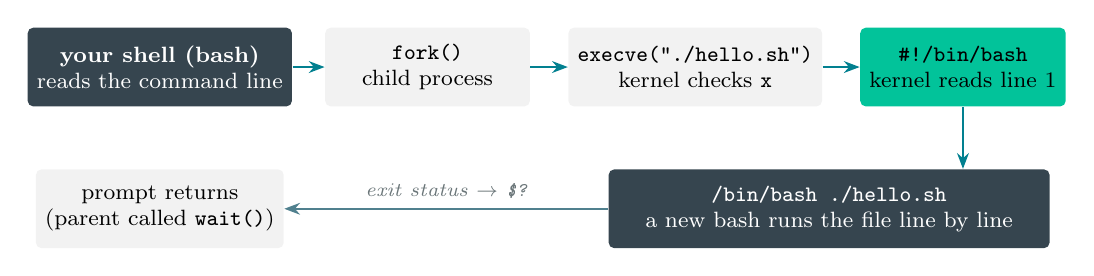
\begin{tikzpicture}[b/.style={rectangle,rounded corners=2pt,minimum height=1.0cm,minimum width=2.6cm,align=center,font=\footnotesize},
  arr/.style={-{Stealth[length=2mm]},thick,mintdeep}]
\node[b,fill=charcoal,text=white] (sh) at (0,0) {\textbf{your shell (bash)}\\reads the command line};
\node[b,fill=light] (fk) at (3.4,0) {\texttt{fork()}\\child process};
\node[b,fill=light] (ex) at (6.8,0) {\texttt{execve("./hello.sh")}\\kernel checks \texttt{x}};
\node[b,fill=mint] (sb) at (10.2,0) {\texttt{\#!/bin/bash}\\kernel reads line 1};
\node[b,fill=charcoal,text=white,minimum width=5.6cm] (run) at (8.5,-1.8) {\texttt{/bin/bash ./hello.sh}\\a new bash runs the file line by line};
\node[b,fill=light] (pr) at (0,-1.8) {prompt returns\\(parent called \texttt{wait()})};
\draw[arr] (sh) -- (fk); \draw[arr] (fk) -- (ex); \draw[arr] (ex) -- (sb);
\draw[arr] (sb.south) -- (sb.south |- run.north);
\draw[arr,slate] (run.west) -- node[above,font=\scriptsize\itshape,text=muted]{exit status $\to$ \texttt{\$?}} (pr.east);
\end{tikzpicture}
\caption{Running a script: fork, exec, shebang, a new interpreter process, and the exit status back to the parent.}
\end{figure}

The shell \cmd{fork()}s a child (Week~3), and the child calls \cmd{execve()} on the file. The kernel checks the execute permission (Week~11). A text file is not machine code, so the kernel looks at its first two bytes: \texttt{\#!} means “start the program named on this line and pass it the script's path”. The kernel therefore actually runs \texttt{/bin/bash ./hello.sh}. The parent shell waits; when the script ends, its exit status is returned to the parent and is available as \texttt{\$?}.

\begin{keyidea}[A script runs in a child process]
Variables you set and \cmd{cd} commands you run \emph{inside} a script change only the child process. When the script ends, your terminal is exactly where it was. (To run a file inside the \emph{current} shell, use \cmd{source file} or \cmd{. file}; this is how \texttt{\textasciitilde/.bashrc} is read.)
\end{keyidea}

\subsection{Four ways to run a script}

\begin{center}
\small
\begin{tabular}{@{}llll@{}}
\toprule
\textbf{Command} & \textbf{Needs} & \textbf{Runs in} & \textbf{Typical use}\\
\midrule
`bash hello.sh` & \texttt{r} & a new bash process & quick test, no \texttt{x} bit\\
`./hello.sh` & \texttt{r}+\texttt{x}, shebang & a new process & normal way in this course\\
`hello.sh` & \texttt{r}+\texttt{x}, folder in \texttt{PATH} & a new process & installed tools (e.g.\ in \texttt{\textasciitilde/bin})\\
`source hello.sh` & \texttt{r} & the \emph{current} shell & files that set variables\\
\bottomrule
\end{tabular}
\end{center}

% =====================================================================
\section{Variables, Quoting and Input}

\subsection{Variables}

A variable is created by assignment and used with a \texttt{\$}:
\lstinputlisting[style=out,lastline=7]{../code/out_variables.txt}

The rules are short but strict:
\begin{itemize}
  \item \textbf{No spaces around \texttt{=}.} Bash separates words at spaces, so `name = Ayse` is the command \texttt{name} with the two arguments \texttt{=} and \texttt{Ayse}, hence \texttt{name: command not found}. (On Ubuntu the message is longer because of the \emph{command-not-found} helper; the meaning is the same.)
  \item Names consist of letters, digits and \texttt{\_}, do not start with a digit, and are case-sensitive (\texttt{name} and \texttt{NAME} are different).
  \item `${name}` is the long form; it is needed when letters follow the name: `"${name}s"`.
  \item Every value is text. `count=5` stores the text “5”, not a number; arithmetic needs \texttt{\$(( ))}.
  \item An unset variable is simply empty; bash does not complain.
  \item Convention: UPPERCASE names for environment variables (\texttt{HOME}, \texttt{USER}, \texttt{PATH}, \texttt{SHELL}), lowercase for your own.
\end{itemize}

\subsection{Command substitution and arithmetic}
\label{sec:subst}

\lstinputlisting[style=sh]{../code/variables.sh}
\lstinputlisting[style=out,firstline=12,lastline=16]{../code/out_variables.txt}

\begin{itemize}
  \item \textbf{Command substitution} `$(command)` runs the command and inserts its output (without the final newline). The old form with backquotes does the same but is harder to read and to nest. Note `wc -l < file`: with input redirection (Week~12) \cmd{wc} prints only the number, without the file name --- exactly what we want inside \texttt{\$( )}.
  \item \textbf{Arithmetic expansion} `$((expression))` computes with integers: \texttt{+ - * / \%} and parentheses, with the usual precedence: $3 + 4 \times 2 = 11$ (see the transcript above). Inside, the \texttt{\$} before variable names is optional.
  \item \textbf{Integers only:} $7 / 2$ gives $3$ and $7 \bmod 2 = 1$, because bash uses 64-bit integer arithmetic. For decimals use \cmd{awk} (as in \texttt{report.sh}) or the calculator \cmd{bc}.
\end{itemize}

\subsection{Quoting}
\label{sec:quoting}

\lstinputlisting[style=sh]{../code/quotes.sh}
\lstinputlisting[style=out,firstline=17]{../code/out_variables.txt}

\begin{center}
\small
\begin{tabular}{@{}lll@{}}
\toprule
\textbf{Form} & \textbf{\texttt{\$var}, \texttt{\$( )} expanded?} & \textbf{Spaces kept?}\\
\midrule
\texttt{"double quotes"} & yes & yes --- one word\\
\texttt{'single quotes'} & no, everything is literal & yes --- one word\\
backslash \texttt{\textbackslash\$} & makes \emph{one} character literal & ---\\
no quotes & yes & no --- split into words, \texttt{*} expanded\\
\bottomrule
\end{tabular}
\end{center}

The last two lines of \texttt{quotes.sh} show the most common bug in real scripts. The variable \texttt{file} contains a space. Quoted, \texttt{"\$file"} is one argument and \cmd{wc} counts $2$ lines. Unquoted, the value is split into the two arguments \texttt{final} and \texttt{report.txt}, and \cmd{wc} reports two missing files. \textbf{Rule: put double quotes around every \texttt{\$variable} and every \texttt{\$( )}}, unless you have a reason not to.

The two \texttt{\# shellcheck disable} lines are for \term{ShellCheck}, a free tool (\url{https://www.shellcheck.net}, or \cmd{sudo apt install shellcheck}) that warns about exactly these problems. They tell it that the mistakes are intentional. All other example scripts of this week pass ShellCheck without warnings.

\subsection{Positional parameters}

The words typed after the script name are its \term{arguments}. Inside the script they are \texttt{\$1}, \texttt{\$2}, \ldots:

\lstinputlisting[style=sh]{../code/args.sh}
\lstinputlisting[style=out]{../code/out_args.txt}

\begin{center}
\small
\begin{tabular}{@{}ll@{}}
\toprule
\textbf{Variable} & \textbf{Meaning}\\
\midrule
\texttt{\$0} & the name of the script, as it was typed\\
\texttt{\$1} \ldots\ \texttt{\$9} & the 1st \ldots\ 9th argument (\texttt{\$\{10\}} for the 10th)\\
\texttt{\$\#} & the number of arguments\\
\texttt{"\$@"} & all arguments, each kept as a separate word (use in loops)\\
\texttt{\$*} & all arguments glued into one string\\
\texttt{\$?} & exit status of the last command (Section~\ref{sec:status})\\
\texttt{\$\$} & PID of the current shell (Week~13)\\
\bottomrule
\end{tabular}
\end{center}

The shell splits the command line into words \emph{before} the script starts, so \texttt{"green tea"} arrives as one argument: \texttt{\$\#} is $3$, not $4$. Without arguments, \texttt{\$1} is empty and \texttt{\$\#} is $0$; this is why well-written scripts check \texttt{\$\#} first. The transcript above also contains the last demo of this subsection, \texttt{read}.

\subsection{Keyboard input with \texttt{read}}

\lstinputlisting[style=sh]{../code/greet.sh}

In the transcript the user typed \texttt{Ayse} and \texttt{2006}; the age is $2026 - 2006 = 20$. \cmd{read -r var} waits for one line of input and stores it; \texttt{-p} prints a prompt first; \texttt{-r} keeps backslashes as typed (always use it). With several names, \cmd{read -r first last} splits the line at spaces.

Arguments or \texttt{read}? Arguments are better for automation: \texttt{./grade.sh 72} can be called from another script or from \cmd{cron} with nobody at the keyboard. \texttt{read} is for interactive tools such as menus and games.

% =====================================================================
\section{Exit Status and Tests}
\label{sec:status}

\subsection{Every command answers yes or no}

When a process ends, it returns a small number, its \term{exit status}, to its parent (in C: \cmd{return n} from \cmd{main} or \cmd{exit(n)}, Week~3; the parent collects it with \cmd{wait()}). The shell stores it in \texttt{\$?}:

\lstinputlisting[style=out,lastline=23]{../code/out_status.txt}

\begin{center}
\small
\begin{tabular}{@{}cl@{}}
\toprule
\texttt{\$?} & \textbf{Conventional meaning}\\
\midrule
$0$ & success, “true”\\
$1$ & general failure, “false” (e.g.\ \cmd{grep}: not found)\\
$2$ & wrong usage or serious error (e.g.\ \cmd{ls} of a missing file)\\
$126$ & command found but not executable (Permission denied)\\
$127$ & command not found\\
\bottomrule
\end{tabular}
\end{center}

\begin{keyidea}[0 means success]
In the shell, $0$ is \emph{success} (“true”) and anything from $1$ to $255$ is failure. This is the opposite of C, where $0$ is false. It makes sense: there is one way to succeed, but many ways to fail, and the number can say which.
\end{keyidea}

\texttt{\$?} always refers to the \emph{last} command, so look at it immediately --- the \cmd{echo} itself sets it to $0$ again. \cmd{grep -q} prints nothing at all; it only answers with its exit status, which makes it ideal for decisions.

\subsection{\texttt{test} and \texttt{[ ]}}

\cmd{test} compares numbers, strings or files and answers with its exit status. \texttt{[} is another name for \texttt{test} whose last argument must be \texttt{]}. The transcript shows that \texttt{[} is a shell builtin --- a \emph{command}. This single fact explains every spacing rule: in `[ "$n" -gt 3 ]` the five words \texttt{[}, \texttt{"\$n"}, \texttt{-gt}, \texttt{3}, \texttt{]} are separate arguments of the command \texttt{[}, so they must be separated by spaces. Writing \texttt{[\$n} produces the word \texttt{[5}, which is not a command.

\begin{center}
\small
\begin{longtable}{@{}p{1.6cm}p{2.9cm}p{8.6cm}@{}}
\toprule
\textbf{Type} & \textbf{Operator} & \textbf{True when \ldots\ (example)}\\
\midrule
\endhead
Numbers & \texttt{-eq} \ \texttt{-ne} & equal / not equal: `[ "$n" -eq 0 ]`\\
        & \texttt{-lt} \ \texttt{-le} & less than / less or equal: `[ "$x" -lt 10 ]`\\
        & \texttt{-gt} \ \texttt{-ge} & greater than / greater or equal: `[ "$s" -ge 50 ]`\\
Strings & \texttt{=} \ \texttt{!=} & same text / different text: `[ "$a" = yes ]`\\
        & \texttt{-z} \ \texttt{-n} & string is empty / not empty: `[ -z "$1" ]`\\
Files   & \texttt{-e} & path exists (any type): `[ -e "$p" ]`\\
        & \texttt{-f} \ \texttt{-d} & regular file / directory: `[ -d ~/lab ]`\\
        & \texttt{-r} \ \texttt{-w} \ \texttt{-x} & readable / writable / executable by you\\
        & \texttt{-s} & file exists and is not empty\\
Logic   & \texttt{!} & negation: `[ ! -d "$dir" ]`\\
        & \texttt{\&\&} \ \texttt{||} & and / or between two tests: `[ -f a ] && [ -f b ]`\\
\bottomrule
\end{longtable}
\end{center}

Two traps: numbers are compared with \emph{letters} (\texttt{-lt}, \texttt{-gt}), strings with symbols (\texttt{=}, \texttt{!=}). Inside \texttt{[ ]}, \texttt{<} and \texttt{>} are redirections (Week~12), not comparisons. And \texttt{-eq} compares values while \texttt{=} compares text: `[ 05 -eq 5 ]` is true, `[ 05 = 5 ]` is false. (Bash also offers \texttt{[[ \ldots\ ]]}, a more forgiving keyword; we use the portable \texttt{[ ]}.)

% =====================================================================
\section{Making Decisions: \texttt{if}}

\subsection{The shape of an \texttt{if}}

\begin{lstlisting}[style=sh,numbers=none]
if TEST; then
    commands            # run when TEST succeeds (exit status 0)
elif OTHER_TEST; then
    commands            # optional, as many as you like
else
    commands            # optional: when nothing above succeeded
fi                      # "if" backwards ends the block
\end{lstlisting}
\texttt{TEST} can be \emph{any} command: \texttt{[ \ldots\ ]}, \cmd{grep -q}, \cmd{mkdir}, \ldots. The semicolon before \texttt{then} is needed because \texttt{then} must start a new command; writing \texttt{then} on the next line works as well. Bash tries the tests from top to bottom and runs only the first branch whose test succeeds.

\subsection{Example: \texttt{check.sh}}

\lstinputlisting[style=sh]{../code/check.sh}
\lstinputlisting[style=out,firstline=26]{../code/out_status.txt}

Each kind of path takes a different branch. \texttt{/dev/null} exists (\texttt{-e}) but is a \emph{device file} (Week~9: \texttt{/dev}), so it is neither \texttt{-f} nor \texttt{-d}. The script also shows three good habits: it checks \texttt{\$\#} and prints a \emph{Usage} line; it sends error messages to standard error with \texttt{>\&2} (Week~12), so that \texttt{./check.sh x > out.txt} still shows the error on the screen; and it uses distinct exit codes ($0$ success, $1$ failure, $2$ wrong usage) that a calling script can test.

\subsection{Numeric tests: \texttt{grade.sh}}

\lstinputlisting[style=sh]{../code/grade.sh}
\lstinputlisting[style=out,lastline=10]{../code/out_grade.txt}

The \texttt{elif} tests form a staircase, and their order matters: if \texttt{-ge 50} came first, a score of $92$ would get a C. \texttt{||} means “or”: the second test runs only if the first one failed. (The scale is only an example, not an official grading scale.)

\subsection{Debugging}
\label{sec:debug}

Three tools find most bugs:
\begin{itemize}
  \item \cmd{bash -n script.sh} checks the syntax without running anything (Section~\ref{sec:errors}).
  \item \cmd{bash -x script.sh} prints every command, marked with \texttt{+}, \emph{after} expansion and before it runs. Inside a script, \cmd{set -x} \ldots\ \cmd{set +x} traces only a part.
  \item Reading the error message: it names the script, the \emph{line number} and the word bash could not handle.
\end{itemize}
\lstinputlisting[style=out,firstline=11]{../code/out_grade.txt}

The trace shows that \texttt{\$score} became $72$, that the test \texttt{-ge 85} failed and \texttt{-ge 70} succeeded. The run with \texttt{abc} reveals a real bug: every numeric test complains \texttt{integer expression expected} and counts as false, so the script falls through to \texttt{else} and prints grade F. (Line 9 appears twice because both tests joined by \texttt{||} are tried.) The fix is to validate input before using it, for example
\begin{lstlisting}[style=sh,numbers=none]
if ! echo "$score" | grep -qx '[0-9]\{1,3\}'; then
    echo "Error: not a number: $score" >&2; exit 1
fi
\end{lstlisting}
where \cmd{grep -x} requires the whole line to match one to three digits (Week~12 regular expressions).

% =====================================================================
\section{Loops}

\subsection{\texttt{for}: once for every item}

\lstinputlisting[style=sh]{../code/loops.sh}
\lstinputlisting[style=out,lastline=11]{../code/out_loops.txt}

The general form is \texttt{for VAR in LIST; do \ldots; done}. The list can be:
\begin{itemize}
  \item words written out (\texttt{Istanbul Ankara Izmir}) or the arguments \texttt{"\$@"};
  \item a brace expansion \texttt{\{1..5\}} $\to$ \texttt{1 2 3 4 5} (Week~10). Braces cannot contain variables: \texttt{\{1..\$n\}} does not work; use \texttt{\$(seq 1 "\$n")} or a \texttt{while} loop instead;
  \item a wildcard such as \texttt{\textasciitilde/lab/docs/*.txt}: the shell replaces it by the matching file names. Because the loop variable is quoted (\texttt{"\$f"}), the name \texttt{final report.txt} stays in one piece;
  \item the output of a command, \texttt{\$(command)} (split at spaces and newlines).
\end{itemize}
The output also shows \texttt{1 lines}: a script prints exactly what it is told; printing “1 line” would need an \texttt{if}. Bash also has a C-style loop, \texttt{for ((i = 1; i <= 5; i++))}, used in Lab exercise~16. A wildcard works directly at the prompt too:
\lstinputlisting[style=out,firstline=25]{../code/out_loops.txt}

\subsection{\texttt{while}: as long as a test succeeds}

\lstinputlisting[style=sh]{../code/while.sh}
\lstinputlisting[style=out,firstline=12,lastline=17]{../code/out_loops.txt}

Two patterns cover most uses. A \emph{counter} loop changes its variable in every turn; forget \texttt{n=\$((n - 1))} and the loop never ends (stop it with Ctrl+C, i.e.\ SIGINT, Week~13). A \emph{read loop}, \texttt{while read -r x; do \ldots; done < file}, reads one line per turn because the redirection \texttt{< file} after \texttt{done} feeds the whole loop; at the end of the file \texttt{read} fails and the loop stops. The numbers check out: the $20$ values sum to $11\,325$, and $11\,325 / 20 = 566.25$, which integer arithmetic truncates to $566$. (\texttt{until TEST; do \ldots; done} loops while the test \emph{fails}.)

\subsection{Functions}

\lstinputlisting[style=sh]{../code/functions.sh}
\lstinputlisting[style=out,firstline=18,lastline=24]{../code/out_loops.txt}

A function is a named block of commands, defined before use with \texttt{name() \{ \ldots; \}} and called like a command. Inside it, \texttt{\$1}, \texttt{\$2}, \ldots\ are the \emph{function's} arguments, not the script's. \texttt{local} keeps a variable private to the function. A function's exit status is that of its last command (or set with \texttt{return n}, $0$--$255$), so \texttt{is\_even} can be used directly in an \texttt{if}. To give back \emph{text}, \texttt{echo} it and capture it with \texttt{\$( )}. Why \texttt{local n} on its own line? \texttt{local n=\$(grep \ldots)} would hide \cmd{grep}'s exit status behind that of \texttt{local}.

% =====================================================================
\section{Syntax Reference}

\begin{center}
\small
\begin{longtable}{@{}p{2.3cm}p{8.3cm}p{2.6cm}@{}}
\toprule
\textbf{Structure} & \textbf{Syntax} & \textbf{Remember}\\
\midrule
\endhead
shebang & `#!/bin/bash` & line 1 only\\
variable & `name=value`, `"$name"`, `"${name}s"` & no spaces at \texttt{=}\\
command subst. & `today=$(date +%F)` & output of a command\\
arithmetic & `n=$((n + 1))`, `$((a % b))` & integers only\\
arguments & `$0 $1 ... $9 $# "$@"` & check \texttt{\$\#}\\
input & `read -r -p "Name? " name` & \texttt{-r} always\\
if & `if [ "$n" -gt 0 ]; then ...; elif ...; then ...; else ...; fi` & spaces in \texttt{[ ]}\\
for (list) & `for c in a b c; do echo "$c"; done` & \\
for (range) & `for i in {1..5}; do ...; done` & no variables in \texttt{\{\}}\\
for (files) & `for f in *.txt; do wc -l "$f"; done` & quote \texttt{"\$f"}\\
for (C style) & `for ((i = 0; i < 5; i++)); do ...; done` & bash only\\
while & `while [ "$n" -gt 0 ]; do n=$((n - 1)); done` & change the variable\\
read a file & `while read -r line; do ...; done < file` & \texttt{<} after \texttt{done}\\
function & `name() { local x=$1; echo "$x"; }` & define before use\\
and / or & `mkdir -p d && echo ok`;\ `[ -f f ] || exit 1` & short \texttt{if}\\
exit & `exit 0` (success), `exit 1` (failure) & $0$--$255$\\
debugging & `bash -n s.sh` (syntax), `bash -x s.sh` (trace) & \\
\bottomrule
\end{longtable}
\end{center}

\begin{tryit}[Two handy expansions (optional)]
`${var:-default}` gives the value of \texttt{var}, or \texttt{default} if it is empty or unset: \texttt{n=\$\{1:-7\}} means “the first argument, or 7”. Lab exercises 7, 8 and 14 use it. `${#var}` gives the length of the string in \texttt{var}.
\end{tryit}

% =====================================================================
\section{Two Real Automation Scripts}

\subsection{\texttt{backup.sh}: a timestamped archive}

\lstinputlisting[style=sh]{../code/backup.sh}

Line by line:
\begin{itemize}
  \item \texttt{\$HOME/lab} rather than \texttt{\textasciitilde/lab}: a tilde is \emph{not} expanded inside double quotes, \texttt{\$HOME} is.
  \item `date +%Y%m%d_%H%M%S` produces a name such as \texttt{20261012\_143005}: unique (to the second), and sortable, because the year comes first.
  \item `[ ! -d ... ]` stops early with a clear message if the source is missing.
  \item \cmd{mkdir -p} creates the destination if needed and is silent if it exists.
  \item \cmd{tar -czf archive -C dir docs} \textbf{c}reates a g\textbf{z}ip-compressed archive \textbf{f}ile; \texttt{-C} changes into \texttt{\textasciitilde/lab} first, so the paths inside the archive start with \texttt{docs/}. \texttt{if tar \ldots} tests tar's own exit status.
  \item \cmd{tar -tzf} lists the archive; \cmd{grep -vc '/\$'} counts the lines that do \emph{not} end in \texttt{/}, i.e.\ files, not folders; \cmd{du -h \textbar\ cut -f1} keeps only the size.
\end{itemize}

\lstinputlisting[style=out]{../code/out_backup.txt}

Each run creates a new archive (the second run was two seconds later), so nothing is overwritten. The archive holds $7$ files: the six visible documents plus the hidden \texttt{.settings} (\cmd{tar} includes hidden files). \texttt{final report.txt} is archived correctly because every variable is quoted. To restore into a scratch folder without touching your files: \cmd{tar -xzf ../backup/docs\_<stamp>.tar.gz -C /tmp}. With \cmd{cron}, the line \texttt{0 18 * * * \$HOME/lab/scripts/backup.sh} in \cmd{crontab -e} would run the script every day at 18:00 (not exam material). Lab exercise~13 adds the deletion of old backups.

\subsection{\texttt{report.sh}: summarising a log and a CSV file}

\lstinputlisting[style=sh]{../code/report.sh}
\lstinputlisting[style=out]{../code/out_report.txt}

The script reuses the pipelines of Week~12: \cmd{awk '\{print \$7\}'} extracts a field, \cmd{sort \textbar\ uniq -c \textbar\ sort -rn} counts and ranks, \cmd{tail -n +2} skips the CSV header and \cmd{cut -d, -f3} takes the department column. What is new is \cmd{awk} doing \emph{decimal} arithmetic: \texttt{m += \$4} adds up the midterm column, the \texttt{END} block runs once at the end, and \texttt{printf "\%.1f"} prints one decimal. A condition alone, such as \texttt{0.4*\$4 + 0.6*\$5 >= 50}, is an awk \emph{pattern}: awk prints only the lines for which it is true, and \cmd{wc -l} counts them. (The $40/60$ weighting is only an example.)

\begin{example}[Checking the report]
All numbers were recomputed independently in Python from the same files:
\begin{itemize}
  \item $98$ of $300$ requests have a status $\ge 400$: $100 \cdot 98 / 300 = 32.67$, and bash integer arithmetic prints $32$.
  \item \texttt{/index.html} and \texttt{/images/logo.png} both have $33$ requests; only one fits in the top~3, and \cmd{sort} breaks the tie.
  \item Departments: $17 + 11 + 10 + 2 = 40$ students.
  \item Average midterm $66.95$ (printed rounded as $67.0$), average final $65.6$.
  \item $35$ of the $40$ students satisfy $0.4\,m + 0.6\,f \ge 50$.
\end{itemize}
\end{example}

% =====================================================================
\section{Common Errors and What They Mean}
\label{sec:errors}

The script \texttt{code/demo\_errors.sh} creates five broken scripts. Their real error messages:

\lstinputlisting[style=out,lastline=25]{../code/out_errors.txt}

\begin{description}[leftmargin=0pt,itemsep=0.3em]
  \item[Spaces around \texttt{=}] \texttt{name: command not found}. Bash ran a command called \texttt{name}. Note that the script did \emph{not} stop: it went on and printed \texttt{Hello } with an empty variable. Fix: \texttt{name="Ayse"}. The opposite mistake, \texttt{name= Ayse}, runs the command \texttt{Ayse} with an empty variable \texttt{name}.
  \item[No spaces inside \texttt{[ ]}] \texttt{[5: command not found}. Fix: \texttt{if [ "\$n" -gt 3 ]; then}.
  \item[Missing quotes] \texttt{[: =: unary operator expected}. The empty, unquoted \texttt{\$answer} vanished, leaving \texttt{[ = yes ]}. With quotes, \texttt{[ "" = yes ]} is simply false. Unquoted file names with spaces give \texttt{No such file or directory} for each half (Section~\ref{sec:quoting}).
  \item[Missing \texttt{fi}, \texttt{done} or quote] \texttt{syntax error: unexpected end of file}: a block was opened and never closed. \cmd{bash -n} finds this without running the script. The reported line is the \emph{end} of the file; the real mistake is earlier.
  \item[Missing \texttt{chmod +x}] \texttt{Permission denied}, exit status $126$ (Section~\ref{sec:running}).
  \item[Not a number] \texttt{integer expression expected} from \texttt{-lt}, \texttt{-gt}, \ldots\ (Section~\ref{sec:debug}).
\end{description}

\subsection{Windows line endings (CRLF)}

Windows editors end each line with two characters, carriage return and line feed (\texttt{\textbackslash r\textbackslash n}, “CRLF”); Linux uses only \texttt{\textbackslash n}. A script written in Notepad and copied to Linux therefore has an invisible \texttt{\textbackslash r} at the end of every line, which sticks to the last word of the line:

\lstinputlisting[style=out,firstline=26]{../code/out_errors.txt}

\begin{itemize}
  \item \texttt{./win.sh}: the kernel looks for an interpreter literally called \texttt{/bin/bash\textbackslash r}, which does not exist. Bash 5.2 (used here) reports \texttt{cannot execute: required file not found}; older versions of bash (e.g.\ Ubuntu 22.04) report the classic \texttt{/bin/bash\^{}M: bad interpreter: No such file or directory}. Both mean the same thing.
  \item \texttt{bash win.sh} runs, but \cmd{cd} receives the path with a \texttt{\textbackslash r} at its end (shown as \texttt{\$'\ldots\textbackslash r'}) and fails.
  \item \cmd{file} says \texttt{with CRLF line terminators}; \cmd{cat -A} shows each \texttt{\textbackslash r} as \texttt{\^{}M} before the end-of-line mark \texttt{\$}.
  \item Fix: \cmd{sed -i 's/\textbackslash r\$//' win.sh} deletes the \texttt{\textbackslash r} at the end of every line; \cmd{dos2unix win.sh} does the same if installed. In VS Code, click “CRLF” in the status bar and choose “LF”.
\end{itemize}

% =====================================================================
\section{Summary}

\begin{keyidea}[Week 14 in eight sentences]
\begin{enumerate}[leftmargin=1.4em]
  \item A shell script is a text file of commands with \texttt{\#!/bin/bash} on line~1; after \cmd{chmod +x} it runs with \texttt{./script.sh}, in a child process created by fork and exec.
  \item Variables are assigned without spaces (\texttt{name=value}) and used in double quotes (\texttt{"\$name"}); single quotes make everything literal.
  \item \texttt{\$(command)} inserts a command's output, \texttt{\$((expression))} computes with integers.
  \item Arguments arrive as \texttt{\$1} \ldots\ \texttt{\$9}, with \texttt{\$\#} and \texttt{"\$@"}; \texttt{read -r} reads the keyboard.
  \item Every command returns an exit status, $0$ meaning success; \texttt{exit n} sets a script's status.
  \item \texttt{[ ]} is a command that tests numbers (\texttt{-eq -lt -gt} \ldots), strings (\texttt{= != -z}) and files (\texttt{-e -f -d}); \texttt{if / elif / else / fi} chooses a branch.
  \item \texttt{for} loops over words, ranges and files; \texttt{while} repeats while a test succeeds or reads a file line by line; functions name a block of commands.
  \item \texttt{bash -n} and \texttt{bash -x} help debug; quote your variables and save scripts with LF line endings.
\end{enumerate}
\end{keyidea}

% =====================================================================
\Needspace{12\baselineskip}
\section{Glossary}

\begin{description}[leftmargin=0pt,itemsep=0.15em]
  \item[Argument (positional parameter)] A word given after the script name; \texttt{\$1}, \texttt{\$2}, \ldots\ inside the script.
  \item[Arithmetic expansion] \texttt{\$(( ))}: integer calculation by the shell.
  \item[Command substitution] \texttt{\$( )}: replaced by the output of the command inside.
  \item[CRLF] Windows line ending \texttt{\textbackslash r\textbackslash n}; breaks scripts on Linux.
  \item[Exit status] Number $0$--$255$ returned by every command; $0$ = success; in \texttt{\$?}.
  \item[Function] Named block of commands with its own arguments.
  \item[PATH] Variable listing the folders where the shell looks for commands.
  \item[Quoting] Double quotes keep spaces and expand variables; single quotes keep everything literal.
  \item[Shebang] The first line \texttt{\#!interpreter} that tells the kernel which program runs the script.
  \item[Shell script] A text file of shell commands run by an interpreter such as bash.
  \item[test / \texttt{[ ]}] Command that evaluates a condition and answers with its exit status.
\end{description}

% =====================================================================
\section{Try It Yourself}

\begin{tryit}[Explore on your own machine]
\begin{enumerate}[leftmargin=1.4em]
  \item Put \texttt{cd /tmp} and \texttt{pwd} in a script and run it. In which folder is your terminal afterwards? Now run it with \cmd{source}. Explain the difference with Week~13 (processes).
  \item Add \texttt{echo "My PID is \$\$, my parent is \$PPID"} to \texttt{hello.sh}, run it twice, and compare with \cmd{echo \$\$} at the prompt.
  \item Run \cmd{bash -x loops.sh}. How many times is the body of each loop executed?
  \item Make \texttt{grade.sh} reject non-numeric input (use the \cmd{grep -qx} test from Section~\ref{sec:debug}).
  \item If you have \cmd{shellcheck}, run it on \texttt{quotes.sh} after deleting the two \texttt{\# shellcheck} lines. What does it report?
\end{enumerate}
\end{tryit}

% =====================================================================
\section{Review Questions}

\subsection*{Conceptual}
\begin{enumerate}[leftmargin=1.6em]
  \item What does the line \texttt{\#!/bin/bash} do, and who reads it?
  \item Why does \texttt{./hello.sh} need the execute permission while \texttt{bash hello.sh} does not?
  \item A script contains \texttt{cd /tmp}. After it ends, your terminal is still in your home folder. Why?
  \item Explain the difference between \texttt{"\$name"}, \texttt{'\$name'} and \texttt{\$name}.
  \item Why must there be spaces inside \texttt{[ ]}, but no spaces around \texttt{=} in an assignment?
  \item What exit status does a successful command return? What do $126$ and $127$ mean?
  \item When is \texttt{read} the right tool, and when are arguments better?
  \item What does \texttt{bad interpreter} (or \texttt{required file not found}) usually mean for a script copied from Windows, and how do you fix it?
\end{enumerate}

\subsection*{Numerical and practical}
\begin{enumerate}[leftmargin=1.6em,resume]
  \item What does \texttt{echo \$(( (17 + 3) / 6 * 6 ))} print? And \texttt{echo \$(( 17 \% 5 ** 2 ))}?
  \item \texttt{./args.sh "a b" c "" d}: what are \texttt{\$\#}, \texttt{\$1} and \texttt{\$3}?
  \item A \texttt{while} loop starts with \texttt{n=10} and runs \texttt{n=\$((n - 3))} while \texttt{[ "\$n" -gt 0 ]}. How many times does the body run, and what is \texttt{n} at the end?
  \item What do the three tests \texttt{[ 010 -eq 10 ]}, \texttt{[ 010 = 10 ]} and \texttt{[ -z "" ]} return (exit status)?
  \item \texttt{for i in \{1..4\}; do s=\$((s + i * i)); done} with \texttt{s=0}: what is \texttt{s}?
  \item Write one line that prints \texttt{OK} if the folder \texttt{\textasciitilde/lab/backup} exists and \texttt{MISSING} otherwise.
\end{enumerate}

\subsection*{Answers to the numerical and practical questions}
\begin{enumerate}[leftmargin=1.6em,start=9]
  \item $(17+3)/6 = 20/6 = 3$ (integer), $3 \times 6 = 18$. In the second, \texttt{**} (power) binds tighter than \texttt{\%}: $5^2 = 25$ and $17 \bmod 25 = 17$.
  \item $\$\# = 4$ (the empty string \texttt{""} is an argument too), \texttt{\$1} $=$ \texttt{a b}, \texttt{\$3} is empty.
  \item $n$: $10 \to 7 \to 4 \to 1 \to -2$; the body runs $4$ times and $n = -2$ at the end.
  \item $0$ (numerically equal), $1$ (different text), $0$ (the string is empty).
  \item $s = 1 + 4 + 9 + 16 = 30$.
  \item \texttt{[ -d \textasciitilde/lab/backup ] \&\& echo OK || echo MISSING} \ (or an \texttt{if}/\texttt{else}/\texttt{fi}).
\end{enumerate}

% =====================================================================
\section{Looking Ahead: Week 15}

\begin{itemize}
  \item \textbf{Week 15: Final exam review.} The final covers the whole course: the theory of Weeks~1--7 (use the Week~8 study guide) and the practical Linux weeks~9--14 --- navigation, file operations, permissions, text processing and pipelines, processes and job control, and shell scripting.
  \item Expect “write the command / pipeline / script” questions: the Lab Sheet above is the best preparation.
  \item The exam date, time and room will be announced on the course Telegram channel.
\end{itemize}

\subsection*{Further reading (optional)}
\begin{itemize}
  \item A.\ Silberschatz, P.\,B.\ Galvin and G.\ Gagne, \emph{Operating System Concepts}, 10th ed., Wiley: Section~2.2 (user and operating-system interface: command interpreters, shells) and Section~3.3 (process creation with \texttt{fork()} and \texttt{exec()}).
  \item R.\,H.\ and A.\,C.\ Arpaci-Dusseau, \emph{Operating Systems: Three Easy Pieces}, Chapter~5, “Interlude: Process API” (how a shell uses fork, exec and wait): \url{https://pages.cs.wisc.edu/~remzi/OSTEP/cpu-api.pdf}
  \item GNU Bash Reference Manual: \url{https://www.gnu.org/software/bash/manual/bash.html}
  \item W.\ Shotts, \emph{The Linux Command Line}, Part~4 “Writing Shell Scripts” (free PDF): \url{https://linuxcommand.org/tlcl.php}
  \item ShellCheck, finds bugs in shell scripts: \url{https://www.shellcheck.net}
\end{itemize}

% =====================================================================
\section{Lab Sheet: Graded Script-Writing Exercises}

Write each script in \texttt{\textasciitilde/lab/scripts}, starting from a fresh lab folder (\cmd{bash \textasciitilde/mcmp117\_lab\_setup.sh}). Every script must start with \texttt{\#!/bin/bash}, have a comment line saying what it does, be executable, pass \cmd{bash -n}, and quote its variables. Name them \texttt{exNN\_name.sh} as shown. In class, exercises 2, 6, 11 and 13 are done and graded (slide “In-Class Lab”); the rest are homework and exam practice. Total: $100$ points. Suggested rubric for each exercise: runs without errors $40\%$, correct output $30\%$, handles bad input $15\%$, style (comments, quoting, shebang) $15\%$.

\subsection*{Part A --- Basics (5 points each)}
\begin{enumerate}[leftmargin=1.6em]
  \item \textbf{\texttt{ex01\_myinfo.sh}} Print your user name, your home folder, today's date as \texttt{YYYY-MM-DD}, your login shell, and the number of students in \texttt{\textasciitilde/lab/data/students.csv} (lines minus the header).
  \item \textbf{\texttt{ex02\_power.sh N}} Print $N$, $N^2$ and $N^3$. Without exactly one argument print a Usage line to stderr and exit with status $2$.
  \item \textbf{\texttt{ex03\_hello\_name.sh NAME [CITY]}} Print \texttt{Hello NAME from CITY!}; if no city is given, use Istanbul; if no name is given, print a Usage line and exit $1$.
  \item \textbf{\texttt{ex04\_calc.sh}} Read two integers with \texttt{read} and print their sum, difference, product, and integer quotient with remainder. Refuse to divide by zero.
\end{enumerate}

\subsection*{Part B --- Decisions and simple loops (6 points each)}
\begin{enumerate}[leftmargin=1.6em,resume]
  \item \textbf{\texttt{ex05\_sign.sh N}} Say whether $N$ is positive, negative or zero, and whether it is even or odd.
  \item \textbf{\texttt{ex06\_what.sh PATH\ldots}} For every argument print \emph{file} (with its line count), \emph{directory} or \emph{missing}. Exit with status $1$ if at least one path is missing, else $0$.
  \item \textbf{\texttt{ex07\_table.sh [N]}} Print the multiplication table $N \times 1$ \ldots\ $N \times 10$ (default $N = 7$) with a \texttt{for} loop.
  \item \textbf{\texttt{ex08\_sum.sh [N]}} Compute $1 + 2 + \cdots + N$ with a \texttt{while} loop (default $N = 100$) and compare with the formula $\frac{N(N+1)}{2}$.
\end{enumerate}

\subsection*{Part C --- Files and data (7 points each)}
\begin{enumerate}[leftmargin=1.6em,resume]
  \item \textbf{\texttt{ex09\_doclines.sh}} For every \texttt{.txt} file in \texttt{\textasciitilde/lab/docs}, print its name and number of lines; finally print the total and the longest file.
  \item \textbf{\texttt{ex10\_minmax.sh}} Read \texttt{\textasciitilde/lab/data/numbers.txt} with a \texttt{while read} loop and print the count, minimum, maximum, sum and integer average --- without \cmd{sort}.
  \item \textbf{\texttt{ex11\_levels.sh}} Count the \texttt{INFO}, \texttt{WARN} and \texttt{ERROR} lines of \texttt{\textasciitilde/lab/logs/system.log} with a \texttt{for} loop and \cmd{grep -c}, and print each count as a percentage of all lines.
  \item \textbf{\texttt{ex12\_temp.sh}} Write a function \texttt{c2f} that converts Celsius to Fahrenheit, $F = \frac{9}{5}C + 32$, and print a table for $-10, 0, 10, \ldots, 40$\,°C.
\end{enumerate}

\subsection*{Part D --- Challenge (7 points each)}
\begin{enumerate}[leftmargin=1.6em,resume]
  \item \textbf{\texttt{ex13\_backup\_keep.sh}} Extend \texttt{backup.sh} so that only the $3$ newest archives in \texttt{\textasciitilde/lab/backup} are kept; print the name of every archive it deletes. Test it by running it five times, one second apart.
  \item \textbf{\texttt{ex14\_guess.sh [SECRET]}} A guessing game: the secret is a number from $1$ to $100$ (the argument, or random with \texttt{\$RANDOM}); read guesses until the right one, answer \emph{Too small} / \emph{Too big}, and finally print the number of tries.
  \item \textbf{\texttt{ex15\_dept.sh DEPT}} Print the number of students and the average final grade (one decimal) of one department from \texttt{students.csv}; exit $1$ with a message for an unknown department.
  \item \textbf{\texttt{ex16\_status\_bars.sh}} For every HTTP status code in \texttt{access.log} print the code, its count and a bar with one \texttt{\#} per $5$ requests (rounded down).
\end{enumerate}

\textbf{Points:} $4 \times 5 + 4 \times 6 + 8 \times 7 = 20 + 24 + 56 = 100$.

% =====================================================================
\section{Lab Sheet Solutions}

These solutions are in \texttt{code/solutions/}. Each was run with bash~5.2 in a fresh lab folder and passes \cmd{bash -n} and ShellCheck; the outputs are real (file \texttt{code/solutions/out\_solutions.txt}). Other correct solutions are of course possible. Try first, then compare!

\lstdefinestyle{solsh}{style=sh,basicstyle=\ttfamily\scriptsize\color{light},aboveskip=0.3em,belowskip=0.2em}
\lstdefinestyle{solout}{style=out,basicstyle=\ttfamily\scriptsize\color{light},aboveskip=0.2em,belowskip=0.4em}
\newcommand{\sol}[4]{\Needspace{6\baselineskip}\par\smallskip{\headfont\bfseries\color{mintdeep}#1}\lstinputlisting[style=solsh]{../code/solutions/#2}\lstinputlisting[style=solout,firstline=#3,lastline=#4]{../code/solutions/out_solutions.txt}}

\sol{1. ex01\_myinfo.sh}{ex01_myinfo.sh}{1}{6}
\sol{2. ex02\_power.sh}{ex02_power.sh}{7}{10}
\sol{3. ex03\_hello\_name.sh}{ex03_hello_name.sh}{11}{14}
\sol{4. ex04\_calc.sh}{ex04_calc.sh}{15}{21}
\sol{5. ex05\_sign.sh}{ex05_sign.sh}{22}{27}
\sol{6. ex06\_what.sh}{ex06_what.sh}{28}{33}
The variable \texttt{status} remembers a failure while the loop continues with the other arguments.
\sol{7. ex07\_table.sh}{ex07_table.sh}{34}{44}
\sol{8. ex08\_sum.sh}{ex08_sum.sh}{45}{47}
Check: $\frac{100 \cdot 101}{2} = 5050$.
\sol{9. ex09\_doclines.sh}{ex09_doclines.sh}{48}{55}
\texttt{printf '\%-18s \%3d'} prints the name left-aligned in $18$ columns and the number right-aligned in $3$. Total: $2 + 5 + 1 + 1 + 1 + 15 = 25$.
\sol{10. ex10\_minmax.sh}{ex10_minmax.sh}{56}{57}
The first number initialises both \texttt{min} and \texttt{max}. Same sum as \texttt{while.sh}: $11\,325$, average $566$ (integer).
\sol{11. ex11\_levels.sh}{ex11_levels.sh}{58}{61}
$79 + 28 + 13 = 120$. The percentages add up to $98\%$, not $100\%$, because integer division truncates ($65.8 \to 65$, $23.3 \to 23$, $10.8 \to 10$). The spaces in \texttt{" \$level "} make sure only the level column matches.
\sol{12. ex12\_temp.sh}{ex12_temp.sh}{62}{69}
For multiples of $5$, $9C/5$ is an integer, so the integer result is exact: $40 \cdot 9 / 5 + 32 = 104$.
\sol{13. ex13\_backup\_keep.sh}{ex13_backup_keep.sh}{70}{79}
\cmd{ls -1t} lists the archives newest first; \cmd{tail -n +4} skips the three newest and passes the rest to the loop. \textbf{Careful:} \cmd{rm} has no recycle bin (Week~10). Test such a script on copies first, and print what you delete. Parsing \cmd{ls} output is safe here only because the names contain no spaces.
\sol{14. ex14\_guess.sh}{ex14_guess.sh}{80}{86}
The player typed $50$, $25$ and $37$. With a fixed secret the game is testable; without an argument, \texttt{\$RANDOM \% 100 + 1} gives $1$--$100$.
\sol{15. ex15\_dept.sh}{ex15_dept.sh}{87}{92}
\cmd{grep -cx} counts lines that match the \emph{whole} department name; \texttt{awk -v d=\ldots} passes the shell variable into awk. Check: ECT finals sum to $1072$, $1072/17 = 63.06$.
\sol{16. ex16\_status\_bars.sh}{ex16_status_bars.sh}{93}{99}
\texttt{while read -r count code} splits each line of \cmd{uniq -c} into two variables. Check: $148/5 = 29.6 \to 29$ characters; the counts sum to $300$.

\end{document}
